% Created 2021-01-07 Thu 12:43
% Intended LaTeX compiler: pdflatex
\documentclass[presentation]{beamer}
\usepackage[utf8]{inputenc}
\usepackage[T1]{fontenc}
\usepackage{graphicx}
\usepackage{grffile}
\usepackage{longtable}
\usepackage{wrapfig}
\usepackage{rotating}
\usepackage[normalem]{ulem}
\usepackage{amsmath}
\usepackage{textcomp}
\usepackage{amssymb}
\usepackage{capt-of}
\usepackage{hyperref}
\usetheme{UoB}
\author{Mark Blyth}
\date{}
\title{Plan of action, brute force testing}
\hypersetup{
 pdfauthor={Mark Blyth},
 pdftitle={Plan of action, brute force testing},
 pdfkeywords={},
 pdfsubject={},
 pdfcreator={Emacs 27.1 (Org mode 9.3)}, 
 pdflang={English}}
\begin{document}

\maketitle

\section{Background}
\label{sec:orgf581752}
\begin{frame}[label={sec:org8d378d7}]{Things I did}
\begin{itemize}
\item Collocation
\begin{itemize}
\item Coded up numerical continuation with collocation
\item Redesigned collocation equations for BSplines
\item Coded up BSpline numerical continuation
\end{itemize}
\end{itemize}
\vfill
\begin{itemize}
\item Planning
\begin{itemize}
\item Reviewed all the work on discretisations so far, for inspiration
\item Drew up a loose plan for the year
\end{itemize}
\end{itemize}
\vfill
\begin{itemize}
\item Testing
\begin{itemize}
\item Systematically tested lots of combinations of control gain, solver, discretisation
\item Discovered probable cause of spline failure
\end{itemize}
\end{itemize}
\end{frame}

\section{Plan}
\label{sec:org2b1b187}
\begin{frame}[label={sec:orgd768e16}]{Overall PhD goal}
Goal: use CBC to classify bursting neurons by slow/fast analysis
\vfill
\begin{itemize}
\item There's lots of burster types, classified by their fast-subsystem singularity and codimension
\item Krasi showed that a cubic Lienard model describes many burster fast-subsystems
\item Possible way to classify\ldots{}
\begin{itemize}
\item Map out the critical manifold \emph{[hard!]}
\item Produce a bifurcation diagram of the fast subsystem
\item Fit the cubic Lienard model from the results
\item Use that to classify the neuron
\end{itemize}
\end{itemize}
\vfill
Combines CBC, multiple timescale analysis, and system identification in a \emph{[hopefully]} biologically useful way
\end{frame}

\begin{frame}[label={sec:org3dad4d5}]{Overall PhD goal}
\begin{itemize}
\item Key challenge: separating out the fast and slow subsystems
\begin{itemize}
\item With models, we can separate equations into fast and slow components
\item This reveals critical manifold and its bifurcations
\item No obvious way of doing this experimentally, would require other approaches
\item If this can be done it would potentially be a big result
\end{itemize}
\end{itemize}
\vfill
Questions for Krasi:
\begin{itemize}
\item This is mathematically interesting, but is it biologically interesting / useful?
\begin{itemize}
\item Where has burster classification been useful to biologists?
\end{itemize}
\item How complex are \emph{real} burster dynamics?
\begin{itemize}
\item There's a lot of complicated multiple-timescale dynamics (torus canards, MMOs) available in neuron models
\item Are these dynamics just mathematical toys, or are they seen in live cells too?
\end{itemize}
\end{itemize}
\end{frame}

\begin{frame}[label={sec:orgebe8d45}]{High-level year plan}
\begin{itemize}
\item Paper 1: get BSpline discretisation working; target: done by March
\end{itemize}
\vfill
\begin{itemize}
\item Paper 2: a set of extensions that didn't make it to paper 1; target: done by May
\begin{itemize}
\item Try some other discretisation methods, since most of the work is done for them
\item Create a recipe book of which discretisation to use when
\item Demonstrate the discretisations on any existing CBC rig?
\end{itemize}
\end{itemize}
\vfill
\begin{itemize}
\item Then, investigate multiple-timescale analysis, nonlinear model identification, and active learning; rest of the year?
\end{itemize}
\end{frame}
\begin{frame}[label={sec:org7902545}]{Plan: immediate}
\begin{itemize}
\item Test results suggest that adaptive stepsizes might be the secret to splines success
\item TODO: implement and test adaptive stepsizes
\end{itemize}
\end{frame}

\begin{frame}[label={sec:orgd35567d}]{Plan: month}
Assuming stepsizes solves all the problems\ldots{}
\vfill
\begin{itemize}
\item Try wavelets in place of BSplines
\begin{itemize}
\item \emph{Should} be quick and easy
\end{itemize}
\item Look into adaptive\ldots{}
\begin{itemize}
\item Knots for BSplines
\item Number of knots?
\end{itemize}
\item Demonstrate results on some prototypical systems and write up into a paper
\end{itemize}
\vfill
Aim to start writing up by the end of January
\end{frame}

\begin{frame}[label={sec:org96bf7f4}]{Plan: exensions}
\begin{itemize}
\item Collocation codes could be used with CBC easily
\item Maybe try some novel CBC approaches
\begin{itemize}
\item Collocation discretisation
\item LSQ collocation
\item Bayesian opimization as a surrogate solver
\end{itemize}
\end{itemize}
\vfill
\begin{itemize}
\item Solves similar problems to BSpline/Wavelets paper so its less useful
\item \ldots{}but lots of the work for this is done, so it could be easy extra paper
\item These ideas hopefully won't take much time to test
\begin{itemize}
\item Test alongside writing up previous stuff
\end{itemize}
\end{itemize}
\end{frame}

\begin{frame}[label={sec:org7e7649f}]{Collocation and BayesOpt}
\begin{itemize}
\item If we have more collocation points than coefficients, we can fit coefficients in a LSQ sense
\begin{itemize}
\item More numerical robustness: guarantees CBC solution exists, even if discretisation is inexact
\item More noise-robustness: noise is averaged off by LSQ
\end{itemize}
\end{itemize}
\vfill
\begin{itemize}
\item Alternative: use Bayesian optimization to minimise \(\|\text{target}(t)-\text{output}(t)\|\)
\begin{itemize}
\item Bayesian optimization is basically a surrogate method
\item Accuracy: gets results fast even with higher-dimensional discretisations
\item Robustness: noise is explicitly modelled, and averaged off
\end{itemize}
\end{itemize}
\vfill
Might make a nice paper or conference paper
\end{frame}

\begin{frame}[label={sec:orga3462ec}]{Another possible extension}
Lots of novel discretisations available
\begin{itemize}
\item Wavelets
\item BSplines
\item Collocation
\item BayesOpt
\end{itemize}
\vfill 
Test them out with CBC\ldots{}
\begin{itemize}
\item In the presence of noise
\item In experiments, on any available, existing CBC rigs
\end{itemize}
\vfill 
Possible outcomes: 
\begin{itemize}
\item A `recipe book' of which discretisor to choose when
\item An adaptive method that automatically chooses the best discretisation at each predictor/corrector step
\end{itemize}
\end{frame}

\begin{frame}[label={sec:orge89b414}]{Plan: beyond discretisation}
Look into slow/fast systems, and nonlinear model identification
\vfill
\begin{itemize}
\item Use a CBC bifurcation diagram to propose system models
\item Link CBC directly into the model generation
\begin{itemize}
\item Active learning procedure
\item Model identification routine decides what data will be most informative at each step
\item CBC is used to obtain that information
\end{itemize}
\end{itemize}
\vfill
Hopefully start this in spring, after discretisors are done
\begin{itemize}
\item Start some reading now!
\end{itemize}
\end{frame}
\section{Exhaustive testing}
\label{sec:orga95c3a4}
\begin{frame}[label={sec:org8b83fa3}]{Brute force testing}
\begin{itemize}
\item Collocation was motivated by some numerical quirks with BSplines
\end{itemize}
\vfill
\begin{itemize}
\item Decided to systematically test control gain, solver, discretisation, to see exactly what quirks arise when
\begin{itemize}
\item Could also have varied discretisation size, but that's never seemed to have much of an impact with Duffing data
\end{itemize}
\end{itemize}
\vfill
\begin{itemize}
\item Shows what the quirks are and where they arise
\begin{itemize}
\item Conclusion: use adaptive stepsizes
\end{itemize}
\end{itemize}
\end{frame}

\begin{frame}[label={sec:org4869f2e}]{Controllers: what and why?}
\alert{Key takeaway: fails at basically the same place, in the same way, regardless of \(K_p\), suggesting that the issues aren't down to the controller or controllability}
\vfill
Can't solve the IO-map if we can't control the system, so \(K_p\) is worth testing
\vfill
\begin{itemize}
\item I'd expect low \(K_p\) to not work: too small means we can't control the system; \emph{agrees with results}
\item I'd expect large \(K_p\) to not work: too big means negligable proportional error, negligable gradient in solution-neighbourhood, so hard to solve accurately and to spot when control is noninvasive; \emph{agrees with results}
\item I'd expect a wide range of middle-ground \(K_p\), as tested, to work; \emph{agrees with results}
\end{itemize}
\end{frame}

\begin{frame}[label={sec:org1916d2c}]{Controllers: what and why?}
Results conform to expectations, suggesting no need for fancier control strategies here
\vfill
Interesting project for someone: what's the best control strategy?
\begin{itemize}
\item Strong enough control to steer the system properly
\item Gentle enough control for the continuation equations to remain numerically solvable
\item Can we always find a \(K_p\) sweetspot?
\end{itemize}
\end{frame}

\begin{frame}[label={sec:orge949b7b},plain]{Solvers: what and why?}
\alert{Key takeaway: no concerning differences between different solvers, suggesting they're not at fault}
\vfill
\begin{itemize}
\item Both solvers should get basically the same solution
\begin{itemize}
\item Noninvasive control is noninvasive control, regardless of how we find it
\item Might expect to see a little difference between SciPy and DIY solver; DIY solver uses fixed finite-differences stepsizes; SciPy solver will be more clever, more accurate
\end{itemize}
\end{itemize}
\vfill
\begin{itemize}
\item Both solvers struggle on second stable branch with BSplines
\begin{itemize}
\item SciPy solvers give up at same place as Newton accepts incorrect solutions
\item It looks like they're failing in the same places; SciPy knows its failing, Newton doesn't
\item Reassuring: suggests success or failure is reasonably solver-indepenent
\end{itemize}
\end{itemize}
\vfill
\begin{itemize}
\item Matches previous results; can't always get a spline solution 
\begin{itemize}
\item Previous suggestion: maybe a solution doesn't exist
\item New suggestion: maybe this a numerical, rather than existence-and-uniqueness, issue?
\end{itemize}
\end{itemize}
\end{frame}

\begin{frame}[label={sec:orgbcaaf11}]{Discretisors: what and why?}
\begin{itemize}
\item Ideally we would expect near-identical results between Fourier and splines
\begin{itemize}
\item Noninvasive control is noninvasive control, regardless of whether it's expressed with splines or Fourier
\end{itemize}
\item Generally this seems to be true
\begin{itemize}
\item I expect the differences in discretisor actually arise from the different stepsize requirements
\end{itemize}
\item Comparing discretisors is slightly tricky
\begin{itemize}
\item Ideally we want to keep everything the same except the discretisor
\item Different stepsizes will work best for different discretisations, so it's hard to do a like-for-like comparison
\item This reveals something interesting!
\end{itemize}
\end{itemize}
\end{frame}

\begin{frame}[label={sec:orgdeaafd5}]{Stepsizes: what and why?}
\begin{itemize}
\item In the current code, we use a fixed stepsize
\item I'd tried varying stepsizes, with no success
\begin{itemize}
\item Perhaps a small stepsize is required for success in some places, and a large stepsize in others
\item Perhaps choosing big steps will fail on one part of the curve, small steps will fail elsewhere
\item Never saw success when varying stepsizes, maybe because there's no single stepsize that works for the whole curve
\end{itemize}
\end{itemize}
\vfill
 \alert{If true, adaptive stepsizes will fix everything!}
\end{frame}

\begin{frame}[label={sec:org2cb5e8c}]{Summary}
\begin{itemize}
\item Success is reasonably independed of control gain
\begin{itemize}
\item \(K_p\) should be not too big and not too small
\end{itemize}
\item Success is reasonably independent of solvers
\begin{itemize}
\item Main difference is that SciPy will be more accurate when it works, and it knows when it's failed
\end{itemize}
\item Success is reasonably independent of discretisation
\begin{itemize}
\item Spline and Fourier success is down to stepsizes, rather than discretisations
\end{itemize}
\item Success \emph{is} dependent on stepsize!
\begin{itemize}
\item I'd tested stepsize in the past, but with no success
\item Perhaps then, small steps fail in some places, large steps fail in others
\item Adaptive stepsizes might fix everything!
\end{itemize}
\end{itemize}
\end{frame}
\section{Collocation results}
\label{sec:org07e4fa1}
\begin{frame}[label={sec:org7850ca3}]{Orthogonal collocation}
Coded up using the standard collocation method:
\begin{itemize}
\item Express periodic orbit as a BVP, and rescale to unit interval
\item Split interval up into mesh, and model solution as a polynomial within each mesh segment
\item Choose each segment's collocation points as (scaled) zeros of Legendre polynomials
\item Find the polynomial coefficients that
\begin{itemize}
\item exactly solve the BVP at the collocation points;
\item result in continuity between intervals;
\item result in periodicity;
\item also satisfy the phase constraint.
\end{itemize}
\end{itemize}
\end{frame}

\begin{frame}[label={sec:orgf851484},plain]{Results}
\vfill 
It works! Continuing periodic orbits from a Hopf normal form:

\begin{center}
\includegraphics[width=.9\linewidth]{./PO_continuation.pdf}
\end{center}
\end{frame}

\begin{frame}[label={sec:orgd80bfd0}]{Collocation meshs}
Standard continuation uses Lagrange polynomials in each subinterval
\begin{center}
\includegraphics[width=.9\linewidth]{./5_basis.pdf}
\end{center}
\end{frame}

\begin{frame}[label={sec:org047a9f9},plain]{Collocation meshs}
Lagrange coefficients are the value of the polynomial at a set of submesh-points \(\tau_{i,j}\)
\begin{center}
\includegraphics[width=.9\linewidth]{./6_submesh.pdf}
\end{center}
\end{frame}

\begin{frame}[label={sec:org97d3016},plain]{BSpline collocation}
BSPline knots form their own mesh, so we could either
\begin{itemize}
\item Use a set of BSplines within each mesh subinterval, so that the knots define \(\tau_{i,j}\)\ldots{}
\begin{itemize}
\item Solution is made of curve sections, with each curve made of polynomial sections
\end{itemize}
\item \ldots{}or let the BSplines define the mesh \(\tau_i\) and use a single set over the entire interval
\begin{itemize}
\item Solution approximation is piecewise-polynomial between meshpoints, much like with standard continuation
\end{itemize}
\end{itemize}
\vfill
I chose the latter (also done in a BSpline BVP paper)
\begin{itemize}
\item Nearly identical to standard continuation, only we enforce a maximally smooth solution
\item I use a periodic BSpline curve
\begin{itemize}
\item Removes the need for periodicity equations
\end{itemize}
\item Spline curves are maximally smooth
\begin{itemize}
\item Removes the need for the \(Nn\) continuity equations
\end{itemize}
\end{itemize}
\end{frame}

\begin{frame}[label={sec:org07b6c6b}]{BSpline collocation}
\begin{itemize}
\item Find periodic orbits by solving a periodic BVP
\item Rescale BVP to unit interval
\item Place BSpline knots evenly across the interval
\item Add exterior knots to create a periodic BSpline curve
\item Find the BSpline coefficients that
\begin{itemize}
\item exactly solve the BVP at the collocation points;
\item satisfy the phase constraint.
\end{itemize}
\item Choose collocation points as (scaled) zeros of Legendre polynomials
\end{itemize}
\end{frame}

\begin{frame}[label={sec:orgbddb6cf},plain]{Results}
\vfill 
It works! Just as easy to use as standard collocation

\begin{center}
\includegraphics[width=.9\linewidth]{./BSpline_continuation.pdf}
\end{center}
\end{frame}
\section{End}
\label{sec:org2fedddc}
\begin{frame}[label={sec:org2a951e5}]{Next steps}
Current TODO: implement and test adaptive stepsize continuation
\vfill
Also, any idea how I get the funding for NODYCON registration?
\end{frame}

\section{Test results}
\label{sec:orgd144d80}
\begin{frame}[label={sec:org284d33a}]{Splines, SciPy solver, \(K_p=0.25\)}
\begin{center}
\includegraphics[width=.9\linewidth]{./kp0d25_transtime100_scipy.pdf}
\end{center}

Can't control UPO
\end{frame}

\begin{frame}[label={sec:org559b66d}]{Splines, DIY Newton solver, \(k_p=0.25\)}
\begin{center}
\includegraphics[width=.9\linewidth]{./kp0d25_transtime100_newton.pdf}
\end{center}

Bad convergence tolerance means non-solutions are accepted
\end{frame}

\begin{frame}[label={sec:orgabcffb8}]{Fourier, SciPy solver, stepsize=1, \(K_p=0.25\)}
\begin{center}
\includegraphics[width=.9\linewidth]{./kp0d25_transtime100_scipy_fourier.pdf}
\end{center}

Can't converge even to first point on curve
\end{frame}

\begin{frame}[label={sec:orgd3c0327}]{Fourier, SciPy solver, stepsize=0.2, \(K_p=0.25\)}
\begin{center}
\includegraphics[width=.9\linewidth]{./kp0d25_transtime100_scipy_fourier_ss0d2.pdf}
\end{center}

Can't control UPO
\end{frame}

\begin{frame}[label={sec:org4ee8291}]{Splines, SciPy solver, \(K_p=0.5\)}
\begin{center}
\includegraphics[width=.9\linewidth]{./kp0d5_transtime100_scipy.pdf}
\end{center}

Works, but takes a huge final step and misses off a lot of the SPO
\end{frame}

\begin{frame}[label={sec:org5642aa5}]{Splines, DIY Newton solver, \(k_p=0.5\)}
\begin{center}
\includegraphics[width=.9\linewidth]{./kp0d5_transtime100_newton.pdf}
\end{center}

Doesn't converge properly
\end{frame}

\begin{frame}[label={sec:org0a2bd98}]{Fourier, SciPy solver, stepsize=1, \(K_p=0.5\)}
\begin{center}
\includegraphics[width=.9\linewidth]{./kp0d5_transtime100_scipy_fourier.pdf}
\end{center}

Huge steps; convergence fails part way along the second SPO branch
\end{frame}

\begin{frame}[label={sec:org8b1e53a}]{Fourier, SciPy solver, stepsize=0.2, \(K_p=0.5\)}
\begin{center}
\includegraphics[width=.9\linewidth]{./kp0d5_transtime100_scipy_fourier_ss0d2.pdf}
\end{center}

Fails to control UPO
\end{frame}

\begin{frame}[label={sec:org6ddf300}]{Splines, SciPy solver, \(K_p=1\)}
\begin{center}
\includegraphics[width=.9\linewidth]{./kp1_transtime100_scipy.pdf}
\end{center}

Works, but takes a huge final step and misses off a lot of the SPO
\end{frame}

\begin{frame}[label={sec:org044a6c7}]{Splines, DIY Newton solver, \(k_p=1\)}
\begin{center}
\includegraphics[width=.9\linewidth]{./kp1_transtime100_newton.pdf}
\end{center}

Doesn't converge properly
\end{frame}

\begin{frame}[label={sec:org25fd48e}]{Fourier, SciPy solver, stepsize=1, \(K_p=1\)}
\begin{center}
\includegraphics[width=.9\linewidth]{./kp1_transtime100_scipy_fourier.pdf}
\end{center}

Fails to converge properly
\end{frame}

\begin{frame}[label={sec:orga0cbd60}]{Fourier, SciPy solver, stepsize=0.2 \(K_p=1\)}
\begin{center}
\includegraphics[width=.9\linewidth]{./kp1_transtime100_scipy_fourier_ss0d2.pdf}
\end{center}

A perfect success!
\end{frame}

\begin{frame}[label={sec:org1ddb797}]{Splines, SciPy solver, \(K_p=1.25\)}
\begin{center}
\includegraphics[width=.9\linewidth]{./kp1d25_transtime100_scipy.pdf}
\end{center}

Fails to converge to next point
\end{frame}

\begin{frame}[label={sec:orgceb72e3}]{Splines, DIY Newton solver, \(k_p=1.25\)}
\begin{center}
\includegraphics[width=.9\linewidth]{./kp1d25_transtime100_newton.pdf}
\end{center}

Converges, albeit with huge, inaccurate step from the same point SciPy failed
\end{frame}

\begin{frame}[label={sec:orgd2abd0c}]{Fourier, SciPy solver, stepsize=1, \(K_p=1.25\)}
\begin{center}
\includegraphics[width=.9\linewidth]{./kp1d25_transtime100_scipy_fourier.pdf}
\end{center}

Continuation finishes early due to convergence failure
\end{frame}

\begin{frame}[label={sec:org5650e9a}]{Fourier, SciPy solver, stepsiez=0.2, \(K_p=1.25\)}
\begin{center}
\includegraphics[width=.9\linewidth]{./kp1d25_transtime100_scipy_fourier_ss0d2.pdf}
\end{center}

Perfect success
\end{frame}

\begin{frame}[label={sec:org37f9252}]{Splines, SciPy solver, \(K_p=1.35\)}
\begin{center}
\includegraphics[width=.9\linewidth]{./kp1d35_transtime100_scipy.pdf}
\end{center}

Continuation terminates early due to convergence failure
\end{frame}

\begin{frame}[label={sec:org8bfb439}]{Splines, DIY Newton solver, \(k_p=1.35\)}
\begin{center}
\includegraphics[width=.9\linewidth]{./kp1d35_transtime100_newton.pdf}
\end{center}

Converges, albeit with huge, inaccurate step from the same point SciPy failed
\end{frame}

\begin{frame}[label={sec:org8f24dec}]{Fourier, SciPy solver, stepsize=1, \(K_p=1.35\)}
\begin{center}
\includegraphics[width=.9\linewidth]{./kp1d35_transtime100_scipy_fourier.pdf}
\end{center}


Continuation finishes early due to convergence failure
\end{frame}

\begin{frame}[label={sec:orgd8b03ff}]{Fourier, SciPy solver, stepsize=0.2, \(K_p=1.35\)}
\begin{center}
\includegraphics[width=.9\linewidth]{./kp1d35_transtime100_scipy_fourier_0d2ss.pdf}
\end{center}

Success
\end{frame}

\begin{frame}[label={sec:org8576fc7}]{Splines, SciPy solver, \(K_p=1.4\)}
\begin{center}
\includegraphics[width=.9\linewidth]{./kp1d4_transtime100_scipy.pdf}
\end{center}

Works, but takes a huge final step and misses off a lot of the SPO
\end{frame}

\begin{frame}[label={sec:org450c46e}]{Splines, DIY Newton solver, \(k_p=1.4\)}
\begin{center}
\includegraphics[width=.9\linewidth]{./kp1d4_transtime100_newton.pdf}
\end{center}

Skips most of the points along second SPO branch
\end{frame}

\begin{frame}[label={sec:org4d6362d}]{Fourier, SciPy solver, stepsize=1, \(K_p=1.4\)}
\begin{center}
\includegraphics[width=.9\linewidth]{./kp1d4_transtime100_scipy_fourier.pdf}
\end{center}

Continuation finishes early due to convergence failure
\end{frame}

\begin{frame}[label={sec:org28c3247}]{Fourier, SciPy solver, stepsize=0.2, \(K_p=1.4\)}
\begin{center}
\includegraphics[width=.9\linewidth]{./kp1d4_transtime100_scipy_fourier_ss0d2.pdf}
\end{center}

Success
\end{frame}

\begin{frame}[label={sec:org53061f6}]{Splines, SciPy solver, \(K_p=1.45\)}
\begin{center}
\includegraphics[width=.9\linewidth]{./kp1d45_transtime100_scipy.pdf}
\end{center}

Fails to converge to even the first point
\end{frame}

\begin{frame}[label={sec:org0138472}]{Splines, DIY Newton solver, \(k_p=1.45\)}
\begin{center}
\includegraphics[width=.9\linewidth]{./kp1d35_transtime100_newton.pdf}
\end{center}

Converges, albeit with huge, inaccurate step 
\end{frame}

\begin{frame}[label={sec:org106d2e2}]{Fourier, SciPy solver, stepsize=1, \(K_p=1.45\)}
\begin{center}
\includegraphics[width=.9\linewidth]{./kp1d45_transtime100_scipy_fourier.pdf}
\end{center}

Continuation finishes early due to convergence failure
\end{frame}

\begin{frame}[label={sec:orga09fe90}]{Fourier, SciPy solver, stepsize=0.2, \(K_p=1.45\)}
\begin{center}
\includegraphics[width=.9\linewidth]{./kp1d45_transtime100_scipy_fourier_ss0d2.pdf}
\end{center}

Success
\end{frame}

\begin{frame}[label={sec:org5c78395}]{Splines, SciPy solver, \(K_p=2\)}
\begin{center}
\includegraphics[width=.9\linewidth]{./kp2_transtime100_scipy.pdf}
\end{center}

Fails to control UPO
\end{frame}

\begin{frame}[label={sec:org23197a1}]{Splines, DIY Newton solver, \(k_p=2\)}
\begin{center}
\includegraphics[width=.9\linewidth]{./kp2_transtime100_newton.pdf}
\end{center}

Fails at the usual place, then accepts non-solutions as the size of their Newton-update step is small
\end{frame}

\begin{frame}[label={sec:org721d969}]{Splines, DIY Newton solver, \(k_p=2\)}
\alert{Zoomed in a bit}
\begin{center}
\includegraphics[width=.9\linewidth]{./kp2_transtime100_newton_zoom.pdf}
\end{center}
\end{frame}

\begin{frame}[label={sec:orgc3d9c8b}]{Fourier, SciPy solver, stepsize=1, \(K_p=2\)}
\begin{center}
\includegraphics[width=.9\linewidth]{./kp2_transtime100_scipy_fourier.pdf}
\end{center}

Continuation finishes early due to convergence failure
\end{frame}

\begin{frame}[label={sec:org2925210}]{Fourier, SciPy solver, stepsize=0.2, \(K_p=2\)}
\begin{center}
\includegraphics[width=.9\linewidth]{./kp2_transtime100_scipy_fourier_ss0d2.pdf}
\end{center}

Success
\end{frame}

\begin{frame}[label={sec:org075ab64}]{Splines, SciPy solver, \(K_p=2.5\)}
\begin{center}
\includegraphics[width=.9\linewidth]{./kp2d5_transtime100_scipy.pdf}
\end{center}

Continuation terminates early due to lack of convergence
\end{frame}

\begin{frame}[label={sec:org1fcdf10}]{Splines, DIY Newton solver, \(k_p=2.5\)}
\begin{center}
\includegraphics[width=.9\linewidth]{./kp2d5_transtime100_newton.pdf}
\end{center}

No idea what's going on here
\end{frame}

\begin{frame}[label={sec:orge75ca48}]{Splines, DIY Newton solver, \(k_p=2.5\)}
\alert{Zoomed in a bit}

\begin{center}
\includegraphics[width=.9\linewidth]{./kp2d5_transtime100_newton_zoom.pdf}
\end{center}

No idea what's going on here
\end{frame}

\begin{frame}[label={sec:orga4286d5}]{Fourier, SciPy solver, stepsize=1, \(K_p=2.5\)}
\begin{center}
\includegraphics[width=.9\linewidth]{./kp2d5_transtime100_scipy_fourier.pdf}
\end{center}

Continuation terminates early due to lack of convergence
\end{frame}

\begin{frame}[label={sec:org1e90107}]{Fourier, SciPy solver, stepsize=0.2, \(K_p=2.5\)}
\begin{center}
\includegraphics[width=.9\linewidth]{./kp2d5_transtime100_scipy_fourier_ss0d2.pdf}
\end{center}

Failed due to lack of convergence
\end{frame}

\begin{frame}[label={sec:orgb4d640e}]{Splines, SciPy solver, \(K_p=2.75\)}
\begin{center}
\includegraphics[width=.9\linewidth]{./kp2d75_transtime100_scipy.pdf}
\end{center}

Fails to converge
\end{frame}

\begin{frame}[label={sec:org3ad0d87}]{Splines, DIY Newton solver, \(k_p=2.75\)}
\begin{center}
\includegraphics[width=.9\linewidth]{./kp2d75_transtime100_newton.pdf}
\end{center}

No idea what's going on here
\end{frame}

\begin{frame}[label={sec:org27f0ffc}]{Splines, SciPy solver, \(K_p=2.75\)}
\begin{center}
\includegraphics[width=.9\linewidth]{./kp2d75_transtime100_scipy_fourier.pdf}
\end{center}

Fails to converge
\end{frame}

\begin{frame}[label={sec:orge6eaa23}]{Fourier, SciPy solver, stepsize=1, \(K_p=2.75\)}
\begin{center}
\includegraphics[width=.9\linewidth]{./kp2d75_transtime100_scipy_fourier.pdf}
\end{center}

Fails to converge
\end{frame}

\begin{frame}[label={sec:orgf86b99a}]{Fourier, SciPy solver, stepsize=0.2, \(K_p=2.75\)}
\begin{center}
\includegraphics[width=.9\linewidth]{./kp2d75_transtime100_scipy_fourier_ss0d2.pdf}
\end{center}

Fails to converge
\end{frame}

\section{How collocation works}
\label{sec:org71e93c2}
\begin{frame}[label={sec:orgf398067}]{}
\begin{center}
Some notes on how collocation works
\end{center}
\end{frame}

\begin{frame}[label={sec:orgee077bd},plain]{How collocation works}
Using the standard collocation method
\begin{itemize}
\item Find LCs by solving a periodic BVP
\begin{itemize}
\item Find a curve that's at some state at time 0, and back at that state at time T
\item State at 0, T forms a boundary value problem
\end{itemize}
\item Rescale BVP to unit interval
\item Split interval up into mesh
\item Model solution as a polynomial within each mesh segment
\item Find the polynomial coefficients that
\begin{itemize}
\item exactly solve the BVP at the collocation points;
\item result in continuity between intervals;
\item result in periodicity;
\item also satisfy the phase constraint.
\end{itemize}
\item Choose collocation points as (scaled) zeros of Legendre polynomials
\end{itemize}

Code was tested on Hopf normal form, as it only handles autonymous systems
\end{frame}

\begin{frame}[label={sec:orgbba6fba},plain]{How collocation works}
Consider a system containing a periodic orbit
\begin{center}
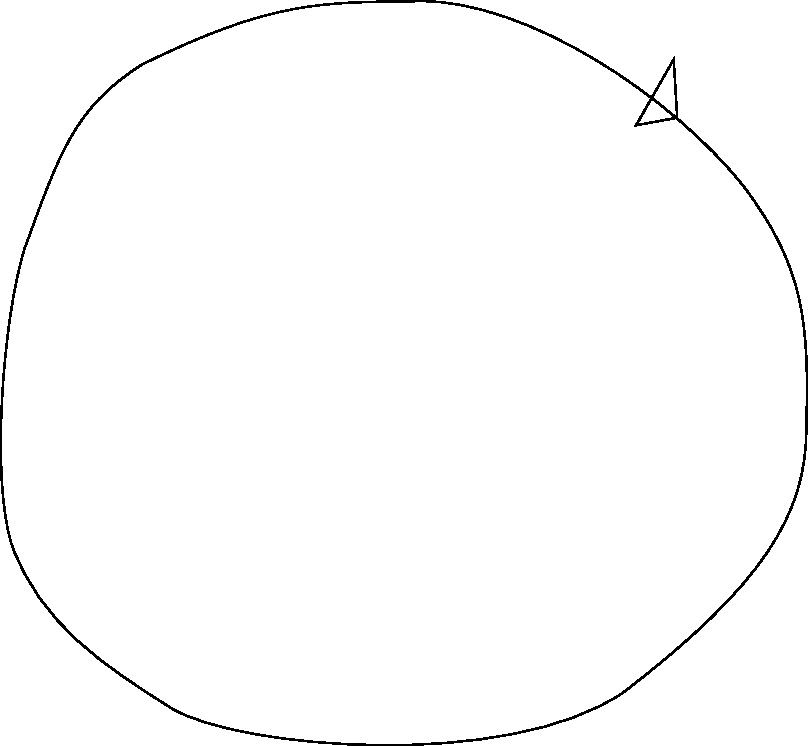
\includegraphics[width=.9\linewidth]{./1_orbit.pdf}
\end{center}
\end{frame}

\begin{frame}[label={sec:orgc55a5e7},plain]{How collocation works}
Cut the orbit at some point; we then have a boundary-value problem
\begin{center}
\includegraphics[width=.9\linewidth]{./2_bvp.pdf}
\end{center}
\end{frame}

\begin{frame}[label={sec:org6a37d6b},plain]{How collocation works}
We now have BVP \(\dot{x} = f(x), \quad x(0)=x(T)\)
\vfill

We could cut anywhere around the orbit, so we choose the cut so that the solution phase is as close as possible to that of some reference \(v(t)\), achieved when
\[\int_0^T\langle x(t), \dot{v}(t)\rangle\mathrm{d}t = 0\]
\vfill
Note that we don't have to explicitly solve for a cut-point; instead, we simply include this constraint within our problem, as a regularisation term.
\end{frame}

\begin{frame}[label={sec:orga4014af},plain]{How collocation works}
Let \(\tau = Tt\).
This rescales the BVP to the unit interval
\begin{center}
\includegraphics[width=.9\linewidth]{./3_rescale.pdf}
\end{center}
\end{frame}

\begin{frame}[label={sec:org088b490},plain]{How collocation works}
Split the BVP domain into a mesh
\begin{center}
\includegraphics[width=.9\linewidth]{./4_mesh.pdf}
\end{center}
\end{frame}

\begin{frame}[label={sec:org2f80dc3},plain]{How collocation works}
Use a set of Lagrange functions to define a polynomial solution approximation over each subinterval
\begin{center}
\includegraphics[width=.9\linewidth]{./5_basis.pdf}
\end{center}
\[u^{(j)}(\tau) = \sum_{i=0}^m u^{j,i} l_{j,i}(\tau)\]
\end{frame}

\begin{frame}[label={sec:orge49dd8e},plain]{How collocation works}
The coefficients \(u_{j,i}\) are the value of the polynomial at a set of submesh-points \(\tau_{i,j}\)
\begin{center}
\includegraphics[width=.9\linewidth]{./6_submesh.pdf}
\end{center}
\end{frame}

\begin{frame}[label={sec:org04be2ca},plain]{How collocation works}
We define a set of collocation points across this subinterval
\begin{center}
\includegraphics[width=.9\linewidth]{./7_coll.pdf}
\end{center}
We require the BVP to be satisfied exactly at each collocation point
\[\sum_i u^{j,i} \dot{l}_{j,i}(\tau) = f(\sum_i u^{j,i} l_{j,i}(\tau) ),\quad \tau = z_{i,j}\]
\end{frame}

\begin{frame}[label={sec:org3a6688d},plain]{How collocation works}
This gives us \(mNn\) equations, for \(m\) collocation points, \(N\) collocation meshpoints, \(n\) dimensions.

We then require continuity between each interval's polynomials, and between the first and last (boundary) points
\begin{center}
\includegraphics[width=.9\linewidth]{./8_continuity.pdf}
\end{center}
\end{frame}

\begin{frame}[label={sec:org411acd1},plain]{How collocation works}
\begin{itemize}
\item This continuity requirement gives us an additional \(Nn\) equations.
\item Finally, we have the periodicity constraint, giving a total of \(mNn + nN + 1\) equations, for \((m+1)Nn\) unknowns \(u^{j,i}\), and one unknown period \(T\).
\item Total of \(mNn + nN + 1\) equations for \(mNn + nN + 1\) unknowns, so we have a fully determined system!
\end{itemize}
\end{frame}

\begin{frame}[label={sec:org7ad56af},plain]{BSpline Collocation}
\begin{itemize}
\item Instead of placing a set of BSplines over every subinterval, we place a single BSpline curve over the entire domain.
\item We choose the BSpline curve to be periodic, which removes the need for the \(Nn\) continuity / periodicity equations.
\item The collocation points are distributed across this interval as usual.
\item We instead have \(n(N-1)\) unknowns, for the BSpline coefficients, and 1 unknown for the period.
\item Choosing \(N-1\) collocation points therefore gives us a full system of equations.
\item In all cases, we choose the collocation points as the zeros of the Legendre polynomial of appropriate degree, rescaled to across the interval.
\end{itemize}
\end{frame}
\end{document}
